\documentclass[a4paper]{article}

\usepackage{float}
\usepackage{url}
\usepackage[margin=1in]{geometry}
\setlength{\parskip}{2ex}
\setlength{\parindent}{0ex}

\usepackage{tikz}
\usetikzlibrary{positioning,calc,fit,arrows,backgrounds}

\usepackage{amsmath, amssymb}
\usepackage{bm}
\usepackage{authblk}
\usepackage[numbers]{natbib}
\bibliographystyle{plainnat}
\usepackage[title, toc, page]{appendix}

\title{Bayesian stochastic model-based forecasting for spatial Covid-19 risk in England \\
Technical Concept Note}

\author[1]{Chris Jewell}
\author[1]{Jonathan Read}
\author[2]{Gareth Roberts}
\author[1]{Barry Rowlingon}
\author[3]{Christopher Suter}
\affil[1]{CHICAS, Lancaster Medical School, Lancaster University, Lancaster, LA1 4YG, UK}
\affil[2]{Department of Statistics, University of Warwick, Coventry, CV4 7AL, UK}
\affil[3]{Google Research, New York}

\begin{document}
\maketitle
\tableofcontents

\newpage
\section{Introduction}

% Up to the data of this report, the COVID-19 outbreak in the UK has demonstrated a marked
% spatial heterogeneity, with a predominance of cases in densely-populated urban centres.
% Capturing this heterogeneity is key to informing effective allocation of behavioural and
% social intervention measures at a local scale, and for optimising the delivery of disease
% surveillance resource across the country.

This document presents a brief description of the Lancaster University ``Spatial Stochastic
Meta-population Model'' for COVID-19 in England, designed to provide locally-resolved
nowcasts and forecasts of case incidence and prevalence, and reproduction number.  The approach makes use of an epidemic
model built around the 317 Local Authority Districts (LADs) in England, using LAD-level
population size and measures of human mobility to explain differences in positive Pillar 1 and 2 tests across the
country in space and time.

Our approach is defined by its capability to formally calibrate the model to
case data, using methodology we have developed during COVID-19.  This builds on our
experience of analogous approaches in real-time modelling of livestock diseases
\citep[e.g.][]{JewEtAl2009b, JewBr2015, PrEtAl2018}, closing a capability gap in applying
such techniques to national human populations.

\paragraph{Caveat} This approach makes use of postive testing data.  Results produced by
this approach are therefore sensitive to fluctuations in case testing due to logistic
constraints.  This caveat must be heeded when interpreting results, and especially if they
are used for policy planning purposes.

\section{Data}

This section describes the 4 sources of data we use to train our model and on which
predictions are subsequently based.

\paragraph{Case data}
The model is calibrated to Public Health England (PHE) Pillar 1 and 2 postive test case reports,
aggregated by day and LAD, for 3 months prior to the analysis date.  The latest 4 days of
data is further discarded, as we observe a consistent recording lag of 4 days\footnotemark.

\paragraph{Inter-LAD connectivity}\label{sec:commute-data}
To establish connectivity between LADs in England, Census 2011 commuting volume data was
aggregated from Middle Super Output Area (MSOA). Two pairs of LADs (Cornwall and Scilly,
and City of Westminster and City of London) were merged to allow
mapping of MSOAs onto LADs.  This reduced the statutory number of LADs from 317 to 315.

Census 2011 provides a matrix of the number of journeys made from
“Residence” to “Workplace” LADs, $W$ of dimension $315 \times 315$.  $W$ is non-symmetric, reflecting
commuting behaviour rather than the reciprocity of disease transmission.  We calculated a
symmetric matrix $W$ of the daily number of journeys between each LAD
$$C = W + W^T$$
assuming that commuters return to their Residence each day, and go from their Residence to
their Workplace and back at most once per day.  We also set
$C_{ii} = 0, \; \mbox{for all}\; i$
as within-LAD infection transmissibility is delegated to another part of our model
(Section \ref{sec:model}).


\paragraph{Traffic volume}\label{sec:traffic-data}
Inter-LAD connectivity data were derived from “business as usual” conditions in
England.   We assume that commuting is modulated during the COVID-19 outbreak by a relative
measure of traffic flow provided by the UK Department for Transport (DfT).  We use this
information to construct a daily timeseries $\bm{w}$\footnotemark[\value{footnote}].

\footnotetext{Data from PHE and DfT are supplied to Lancaster University under a SPI-M-mediated data sharing
agreement.  These data are accessed only by Jewell, Rowlingson, and Read.}

\paragraph{Population size}
The population size $N_i$ for each LAD $i=1,\dots,315$ is taken from ONS Population Size predictions for
December 2019.

\section{Model}\label{sec:model}
 Within each of $m=315$ LADs, we assume the SEIR model in Figure \ref{fig:stm-diagram}
 where at any time $t$, individuals exist in one of
4 disease states: susceptible, exposed (i.e. infected but not yet infectious),
infectious, and finally removed (either solidly immune or dead, Figure
\ref{fig:stm-diagram}).

When susceptible, an individual experiences a ``force of infection''
($\lambda_i(t)$, Figure \ref{fig:stm-diagram}) from
all infectious individuals in its own LAD $i$, as well as infectious individuals in all other
LADs weighted by connectivity $w_t C$:
\begin{equation}
  \lambda_i(t) = \beta_0 e^{\xi_t}\frac{ I_i(t) + \beta_1 w_t C \frac{\bm{I}(t)}{\bm{N}}}{N_i}.
\end{equation}
where $I(t)$ is the vector of numbers of infectious individuals in each LAD, $w_t$ is the
$t$th element of the traffic flow timeseries $\bm{w}$, $C$ is the mobility matrix, and $N$ is
the vector of population size in each LAD. Parameters $\beta_0$, and $\beta_1$
are assumed unknown and must be estimated from data.  $\bm{\xi}$ is similarly unknown, and
represents a 2-week changing baseline force of infection, measuring changes in
transmission in response to unobservable changes in population behaviour.  Individuals
then spend $1/\nu$ days on average in the exposed state, $1/\gamma$ days on average in the
infectious state before becoming removed.  We assume $\nu = 0.5$ to give a 2 day latent
period, and assume $\gamma$ is unknown.

The model is evolved in daily discrete timesteps, using the ``chain binomial'' setup.  For further
technical information, see Appendix \ref{app:data-generating-model}.

\begin{figure} \centering                                                                                           
  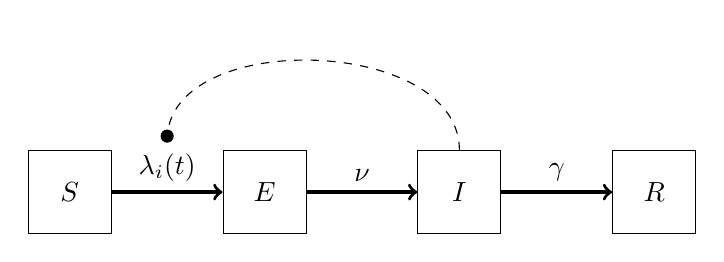
\begin{tikzpicture}[
    auto,
    node distance=40pt,
    box/.style={ draw=black,
      anchor=center,                            
      align=center,
      minimum height=30pt,
      minimum width=30pt}]
    \node[box] (S) {$S$};
    \node[box, right=of S] (E) {$E$};
    \node[box, right=of E] (I) {$I$};
    \node[box, right=of I] (R) {$R$};                          
                                                                                                                     
    \draw[->, very thick] (S) to node (SE) {$\lambda_i(t)$} (E);
    \draw[->, very thick] (E) to node (EI) {$\nu$} (I);
    \draw[->, very thick] (I) to node (IR) {$\gamma$} (R);
    \draw[-*,dashed] (I) to [out=90,in=90,looseness=1] (SE);                                   
                                                                     
   \end{tikzpicture}                                                                                                 
   \caption{SEIR (susceptible, exposed, infectious, removed) model showing transition
     rates.  In particular, the number of infectious individuals feeds back via measures
     of human mobility and proximity into the LAD-specific transition rate $\lambda_i(t)$.}                                                                                      
   \label{fig:stm-diagram}                                                                                           
 \end{figure}


\section{Statistical model fitting}
We fit our model assuming that PHE Pillar 1 and 2 positive tests represent $I\rightarrow
R$ transition events.  Our aim is to estimate unknown parameters $\bm{\theta} = \{ \beta_0, \bm{\xi},
\beta_1, \gamma \}$ in order to subsequently make epidemic predictions forward in time.
Our fitting procedure is based on our previous Bayesian approaches, allowing us to calculate unbiased estimates
for the parameters, allowing for the fact that $S\rightarrow E$ and $E \rightarrow I$
events are not observed \citep{JewEtAl2009b}.

Importantly, the  Bayesian approach fully quantifies uncertainty due to both statistical
uncertainty in parameter estimation and random fluctuations in the epidemic process.  This
provides a natural way to provide uncertainty estimates, for example the probability that
reproduction numbers are greater than unity. For futher details, see Appendix \ref{app:inference}.

\section{Implementation}

The model implementation is written in Python 3.8 using Tensorflow 2.3 (Google Brain) and Tensorflow
Probability 0.14 (Google Research) to make use of GPU-accelerated high performance
computing.  The Python source code is freely available at \url{https://github.com/chrism0dwk/covid19uk}.


\section{Predictions}
Given our model and a fitted posterior distribution over the parameters and censored event
times, we can calculate predictive distributions over a wide range of epidemic metrics of interest.
Specifically, we focus on 3 different aspects:
\begin{description}
\item[Reproduction number] $R_{it}$ is the time-varying reproduction number $R_{it}$ for
LAD $i$ at time $t$ (typically the latest analysis date).  It gives the expected
number of further infections an average individual in that LAD will infect
during its infectious period (both within its own LAD and beyond).  This is a measure of
the capacity of a LAD to generate more cases, should infection arrive into it, and varies
as changes in population behaviour affects disease transmission.

\item[Case incidence] Case incidence $\lambda_{it}$ is the expected rate of new
infections in LAD $i$ at time $t$.  Typically, we quote this as an absolute incidence, in
other words the expected number of cases in total within a LAD given a specified
time-frame.  We do this for resource planning purposes, in order to highlight LADs that
are likely to experience a high number of cases in the short-term based on their current
number of cases.  

\item[Case prevalence] Case prevalence, $\pi_{it}$, gives the expected proportion of
individuals in LAD $i$ who are in \emph{either} the Exposed or Infectious states at time
$t$, i.e. the proportion of individuals who are infected.  This metric may be used to
track the progression of the outbreak in space and time, and captures an overall spatial
measure of how the epidemic is unfolding.
\end{description}

\begin{figure}[H]
  \centering
  \includegraphics[width=0.3\columnwidth]{riskreport_Rt_1.pdf}
  \includegraphics[width=0.3\columnwidth]{riskreport_cases14day_1.pdf}
  \includegraphics[width=0.3\columnwidth]{riskreport_prevalence_2.pdf}
  \caption{Analysis as of 14th September 2020: Estimated reproduction number (left); number of new
    COVID-19 cases by 28th September 2020 (centre); prevalence of COVID-19 on 28th September 2020 (right).}
\end{figure}


\bibliography{bayes_risk}

\newpage

\begin{appendices}
\section{Formal model description}

As described above, we characterise the population within each of $m=315$ LADs into
susceptible, exposed (infected but not yet infectious), infectious, and removed states.
We denote the number of
individuals in each state in LAD $i$ at time $t$ by $S_i(t)$, $E_i(t)$,
$I_i(t)$, $R_i(t)$ respectively, and write $X_i(t) = \{S_i(t), E_i(t), I_i(t), R_i(t)\}$
to denote the overall state of the meta-population.  Since we have $i=1,\dots,m$
LADs, we omit the subscript to denote the state of the entire population, for
example $X(t) = \{X_1(t),\dots,X_m(t)\}$.

As shown in Figure \ref{fig:stm-diagram}, we assume that individuals transition from
susceptible to exposed at rate $\lambda_i(t)$, from exposed to infectious
at rate $\nu$, and from infectious to removed at rate $\gamma$, all rates being in units
of events per day.  We assume that
$\nu$ and $\gamma$ are constant across both meta-populations and time.  Within a LAD, we
assume that the population is well-mixed, and that mixing between LADs is heterogeneous.
The force of infection, $\lambda_i(t)$, is
assumed to vary according to the state of the epidemic and the connectivity between LADs
in a frequency-dependent (i.e. independent of population density) way such that
\begin{equation}
  \lambda_i(t) = \beta_0 e^{\xi(t)} \frac{ I_i(t) + \beta_1 w_t C \frac{\bm{I}(t)}{\bm{N}}}{N_i}.
\end{equation}
with $C$ the zero-diagonal commuting matrix described in Section
\ref{sec:commute-data}, $w_t$ the England-wide relative traffic flow on day $t$
from Section \ref{sec:traffic-data}, and $N$ the vector of population sizes in each
LAD.  Parameters $\beta_0$, $\beta_1$, and $\bm{\xi}$ (which changes every 2 weeks) are
assumed unknown.


\section{Data Generating Process}\label{app:data-generating-model}

Given the characterisation of the SEIR model, the vector of transition rates
$\bm{\lambda}(t)$, onset of infectiousness rate $\nu$,
and removal rate $\gamma$ as defined in Section \ref{sec:model}, we evolve the epidemic in daily time
steps according to a discrete time ``chain-binomial'' Markov process.  Here, the number
of state transitions $Y^{se}_i(t), Y^{ei}_i(t),Y^{ir}_i(t) $ occurring on day $t$ are drawn
from a Binomial distribution conditional on the state $X_i(t)$, i.e.
\begin{eqnarray}\label{eq:chain-binom}
Y^{se}_i(t) & \sim & \mbox{Binomial}(S_i(t), p_{se}) \nonumber \\
Y^{ei}_i(t) & \sim & \mbox{Binomial}(E_i(t), p_{ei}) \nonumber \\
Y^{ir}_i(t) & \sim & \mbox{Binomial}(I_i(t), p_{ir})
\end{eqnarray}
where $p_{se}$, $p_{ei}$, and $p_{ir}$ are the daily probabilities of individuals
undergoing $S\rightarrow E$, $E\rightarrow I$, and $I\rightarrow R$ transitions
respectively given by
\begin{eqnarray*}
  p_{se} & = & 1 - e^{-\bm{\lambda}(t)} \\
  p_{ei} & = & 1 - e^{-\nu} \\
  p_{ir} & = & 1 - e^{-\gamma}.
\end{eqnarray*}
Given the entire state at time $t$, $\bm{Y}(t)$, we propagate the epidemic state by
\begin{eqnarray} \label{eq:propagation}
  S_i(t+1) & = & S_i(t) - Y^{se}(t) \nonumber \\
  I_i(t+1) & = & I_i(t) + Y^{se}(t) - Y^{ei}(t) \nonumber \\
  E_i(t+1) & = & E_i(t) + Y^{ei}(t) - Y^{ir}(t) \nonumber \\
  R_i(t+1) & = & R_i(t) + Y^{ir}(t).
\end{eqnarray}

Given an initial state $X(0)$ and parameters $\bm{\theta}=\{ \beta_0, \beta_1, \nu,
\gamma, \bm{\xi}\}$, the data generating process is then given by iterating Equations
\ref{eq:chain-binom} and \ref{eq:propagation} for $t=1,\dots,T$ where $T$ is the final time of interest.


\section{Statistical Inference}\label{app:inference}
Statistical inference is performed on model parameters $\bm{\theta} = \{ \beta_0, \bm{\xi},
\beta_1, \gamma\}$, assuming that $I\rightarrow R$ transitions $Y^{ir}(t)$ are observed on
each day $t$ and are synonymous with Pillar 1 and 2 case reports (with the patient assumed to fully
self-isolate subsequently).  For convenience we fix the $E\rightarrow I$ transition rate
$\nu = 0.5$ (i.e. 2-day latent period), noting that predictive results are relatively
insensitive to this parameter.  Estimation is performed in a Bayesian paradigm using
Markov chain Monte Carlo (MCMC), with the following priors
\begin{eqnarray*}
\beta_0 & \sim & \mbox{Gamma}(1, 1)     \\
\beta_1 & \sim & \mbox{Gamma}(3, 10)    \\
\gamma  & \sim & \mbox{Gamma}(100, 400) \\
\xi     & \sim & MVN(\bm{0}, \Sigma)    \\  
\end{eqnarray*}
where $\Sigma$ is a covariance matrix with Mat\'ern correlation function
$$\Sigma_{ij} = 0.1 \left( 1 + \frac{\sqrt{3}d}{\rho} \right) \exp
\left(-\frac{\sqrt{3}d}{\rho} \right)
$$
with $\rho = 12$ to give a 4-week effective range.


The challenge to inference in this situation is that although
a statistical likelihood function for observing events $\bm{Y}$ given the model parameters
is straightforward from Equation \ref{eq:chain-binom}, we do not observe $S\rightarrow E$
or $E\rightarrow I$ events, i.e.  $Y^{se}(t)$ and $Y^{ei}(t)$ are censored data.  We approach
this problem by extending our previous work in MCMC data augmentation
techniques for individual-level epidemic models in continuous time to the case of
meta-population models in discrete time to suit our application \citep{JewEtAl2009a,
  JewEtAl2009b}.  The MCMC allows us to sample from the joint posterior probability distribution
$\pi(\bm{\theta}, Y^{se}(0{:}T), Y^{ei}(0{:}T) | y^{ir}(0{:}T), X(0))$ where $X(0)$ is the initial
state at the beginning of our epidemic timeseries chosen by single imputation of the initial censored
event times.

Crucially, both $Y^{se}(0{:}T)$ and $Y^{ei}(0{:}T)$ contain two types of
censored event.  Firstly, partially-censored events refer to those for which we have
observed a corresponding removal (i.e. $I\rightarrow R$) event -- we know that the events
exist, but not precisely when they occurred.  Secondly, ``occult'' events refer to
$S\rightarrow E$ and $E\rightarrow I$ events that have happened, but that we are unaware
of because of not having (yet) observed the corresponding $I\rightarrow R$ event.  In the
Bayesian setting, our MCMC treats these quantities as parameters to be estimated jointly
with $\bm{\theta}$, with implementations of Metropolis-Hastings samplers designed to draw
from their conditional posterior distributions.

The MCMC is tuned manually to obtain Metropolis-Hastings acceptance rates of approximately
23\%, and run for 200,000 iterations.  The initial 100,000 iterations are discarded as
burn-in, and the remaining 100,000 iterations are thinned every 20 iterations for 2000
quasi-independent samples from the joint posterior.  These samples are subsequently used
to calculate summary statistics for the epidemic predictions. 

\end{appendices}

\end{document}



